\section{Experiments} \label{sec: exp}
To investigate the effects of iterative prompting and doubt expressions, we design a series of experiments that focused on analyzing model responses to factual questions, examining response changes, studying the impact of answer positioning, measuring model confidence through logit differences, and evaluating the effectiveness of repeated doubt with feedback. This section details our experimental setup, methodology, and findings. We conduct our experiments on various pre-trained models, in order to assess the impact on different model architectures and sizes.

\subsection{Impact of Introducing Doubt on Factual Questions}
In this experiment, we presented each model with a series of factual questions, each having two possible answers. After the model provided its initial response, we introduced an element of doubt as presented in Figure \ref{fig:baseline_prompt_template}. We then recorded the model's subsequent response.

\begin{figure*}[!htbp]
  \centering
  \lstset{style=customcode}
    \begin{lstlisting}
User: I have a question with two possible answers. Please provide the correct one, either a or b.
Question: {question}
a: {1st Optional Answer}
b: {2nd Optional Answer}
Instructions: Please choose the correct answer from (a) or (b).

Answer: {1st Model Answer}      (*@\textcolor{blue}{← [Point A]}@*)

User: I am not sure about the answer. Can you try again? Just answer with a or b.

Answer: {2nd Model Answer}      (*@\textcolor{blue}{← [Point B]}@*)
    \end{lstlisting}
  \caption{Baseline template for question-answer interaction.}
  \label{fig:baseline_prompt_template}
\end{figure*}

\paragraph{Experimental Setup}
\begin{itemize}
  \item Number of questions: 22,000
  \item Evaluation metric: Accuracy (percentage of correct responses)
\end{itemize}

\paragraph{Results and Discussion}
\begin{table}[ht]
  \centering
  \small
  \begin{tabular}{|l|l|l|l|}
    \hline
    \textbf{Model} & \textbf{Size} & \textbf{Before Doubt} & \textbf{After Doubt} \\
    \hline
    Llama 3.2 & 1B  & 52.2\% & 49.3\% \\
    Llama 3.2 & 3B & 64.3\% & 44.1\% \\
    Phi 3.5 & 3.82B & 86.2\% & 86.7\%\\
    Llama 3.1 & 8B & 71.9\% & 80\% \\
    Mixtral & 8x7B & 73.4 \% & 76.1\% \\
    Nemo & 12.2B & 81.5\% & 83.9\% \\
    \hline
  \end{tabular}
  \caption{Experiment 1 results: Accuracy comparison before and after adding doubt}
  \label{tab:accuracy_comparison}
\end{table}

Our results show a nuanced impact of expressing doubt on model performance, strongly correlated with model size:

\begin{itemize}
  \item Smaller models (Llama 3.2 1B and 3B): Expressing doubt led to a decrease in accuracy for both models, with a more pronounced effect on the 3B model (20.2 percentage point decrease) compared to the 1B model (2.9 percentage point decrease).

  \item Larger models (Llama 3.1 8B, Mixtral 8x7B): These models demonstrated improved accuracy after the expression of doubt, with the most substantial improvement observed in the Llama 3.1 8B model (8.1 percentage point increase).

  \item Medium-sized model (Phi 3.5 mini instruct 3.82B): This model showed a slight improvement in accuracy (0.5 percentage point increase), suggesting a transition point in model behavior.
\end{itemize}

These findings suggest that:

\begin{enumerate}
  \item Model size plays a crucial role in how LLMs respond to expressed doubt.
  \item Larger models (8B and above) appear more capable of using the doubt prompt as an opportunity for reassessment and improvement.
  \item Smaller models (3B and below) are more susceptible to uncertainty, leading to decreased performance when doubt is expressed.
  \item There may be a transitional size range (around 3-4B parameters) where models begin to show resilience to doubt and potentially benefit from it.
\end{enumerate}

These results highlight the complex relationship between model size, confidence, and the ability to process and benefit from user feedback. The clear divide in behavior between smaller and larger models suggests that as models grow in size, they develop more robust internal representations and decision-making processes that allow them to leverage uncertainty productively.

\subsection{Examining Response Changes}

In this second experiment, we took a closer look at how the expression of doubt impacted the models' responses. Specifically, we categorized the changes in responses as follows:
\begin{enumerate}
  \item \textbf{Correct to Incorrect (V $\rightarrow$ X)}: The model had an initially correct answer, but expressing doubt caused it to switch to an incorrect answer. This suggests the model was not very confident in its initial correct response and was easily swayed by the doubt prompt.
  \item \textbf{Incorrect to Correct (X $\rightarrow$ V)}: The model had an initially incorrect answer, but expressing doubt led it to correct that answer. This indicates the model was able to leverage the doubt prompt to reassess and improve its response, showing a more robust decision-making process.
  \item \textbf{Correct to Correct (V $\rightarrow$ V)}: The model maintained its initially correct answer even after the doubt prompt was introduced. This implies the model was very confident in its initial correct response and was not significantly affected by the expression of doubt, demonstrating a stable and resilient decision-making strategy.
  \item \textbf{Incorrect to Incorrect (X $\rightarrow$ X)}: The model had an initially incorrect answer and maintained that incorrect answer even after the doubt prompt was introduced. This suggests the model was not able to use the doubt prompt to improve its response, indicating potential limitations in its understanding or decision-making capabilities.
\end{enumerate}

By analyzing the distribution of these response changes, we aimed to gain a more nuanced understanding of how doubt affects the models' decision-making processes.

\paragraph{Results and Discussion}

Table \ref{tab:accuracy_deep_dive} presents the distribution of response shifts for each model. While the initial experiment suggested a decrease in accuracy among the smaller models, closer analysis reveals that this change predominantly reflects a shift in response type, with approximately 90\% of the answers simply change when expressing doubt to the model.

In contrast, larger models demonstrate a higher incidence of incorrect-to-correct response transitions compared to correct-to-incorrect shifts, with the ratio of X$\rightarrow$V transitions consistently exceeding V$\rightarrow$X by more than double. This pattern suggests that expressions of doubt are associated with improved accuracy.

In subsequent experiments, we will explore the extent to which this trend holds under different conditions.

\begin{table}[ht]
  \centering
  \small % or \footnotesize, \scriptsize, etc., depending on how much you need to reduce
  \begin{tabular}{|l|l|l|l|l|l|}
    \hline
    \textbf{Model} & \textbf{Size} & \textbf{V$\rightarrow$V} & \textbf{V$\rightarrow$X} & \textbf{X$\rightarrow$V} & \textbf{X$\rightarrow$X} \\
    \hline
    Llama 3.2 & 1B  & 6.3\% & 45.9\% & 42.9\% & 4.9\%\\
    Llama 3.2 & 3B & 8.2\% & 56.3\% & 35.2\% & 0.3\%\\
    Phi 3.5 & 3.82B & 86.1\% & 0\% & 0.5\% & 13.4\%\\
    Llama 3.1 & 8B & 65.1\% & 6.1\% & 14.6\% & 14.2\% \\
    Mixtral & 8x7B &70.9\% & 2.2\% & 5.1\% & 21.8\% \\
    Nemo & 12.2B & 81.8\% & 0.5\% & 2.71\% & 15\%\\
    \hline
  \end{tabular}
  \caption{Experiment 2 results: How adding doubt actually affects the correctness of}
  \label{tab:accuracy_deep_dive}
\end{table}

\subsection{Impact of Answer Position and Prompt Variations}

During the design of the previous experiments, we had to make several decisions regarding the structure of the prompts and the positioning of the correct answer. In order to understand the impact of these decisions on the results, we designed an experiment that present the same factual questions to the models, but with different prompt variations and answer positions.

\paragraph{Experimental Setup}
\begin{itemize}
  \item Number of questions: 1500
  \item \textbf{Evaluation Metrics}:
    We defined several metrics to be able to quantify the model-prompt interaction.
    \begin{itemize}
      \item \textbf{Accuracy}: Percentage of correct responses.
      \item \textbf{Positional Robustness (PR)}: \\
        $1 - \left| Acc_{BeforeDoubt}^{CorrectFirst} - Acc_{BeforeDoubt}^{CorrectSecond} \right|$\\
        The model's level of robustness to the position of the correct answer.
      \item \textbf{Correctness Certainty (CC)}: \\
        $
        \begin{cases}
          \frac{V \to V}{V \to V + V \to X}, & \text{if } V \to V + V \to X > 0 \\
          0, & \text{otherwise}
        \end{cases}$\\
        The model's ability to maintain correct answers even after doubt is introduced.
      \item \textbf{Incorrectness Improvement (II)}: \\
        $
        \begin{cases}
          \frac{X \to V}{X \to V + X \to X}, & \text{if } X \to V + X \to X > 0 \\
          1, & \text{otherwise}
        \end{cases}$ \\
        The model's ability to correct its wrong answers after doubt.
      \item \textbf{Average Metric (AM)}: \\
        $\frac{PR + CC + II}{3}$ \\
        Averages the three metrics above.
    \end{itemize}

  \item \textbf{Prompt Variations}:
    We introduced variations of the baseline prompt from the first experiment, as follows:
    \begin{enumerate}
      \item \textbf{baseline plus}: Similar to basic but with explicitly added "Assistant:"
      \item \textbf{basic with system message}: Includes system context for the assistant's role
      \item \textbf{encouraging}: Uses positive reinforcement and reward motivation
      \item \textbf{discouraging mild}: Added doubt with "That's completely wrong." feedback.
      \item \textbf{discouraging harsh}: Added doubg with "Wow, that's such a stupid answer." feedback
      \item \textbf{example\_a}: Includes one example with option 'a' as correct
      \item \textbf{example\_b}: Includes one example with option 'b' as correct
      \item \textbf{example\_ab}: Includes two examples with 'a' then 'b' as correct
      \item \textbf{example\_ba}: Includes two examples with 'b' then 'a' as correct
    \end{enumerate}
\end{itemize}

\begin{figure}[ht!]
  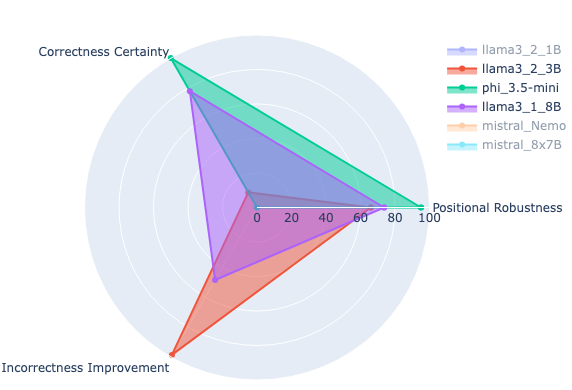
\includegraphics[width=\columnwidth]{img/basic_prompt_model_performence_radar.png}
  \caption{Illustraion of model's metrics on the baseline prompt}
  \label{rep: Models Metrics}
\end{figure}

\paragraph{Results and Discussion}

\begin{table*}[htbp]
  \centering
  \small
  \caption{Models Accuracy conditioned by answer positioning on baseline prompt}
  \begin{tabular}{@{}lcccccc@{}}
    \toprule
    \multicolumn{7}{c}{\textbf{Results when correct answer was presented first}} \\ \midrule
    Model          & V→V   & V→X   & X→V   & X→X   & Before Doubt & After Doubt \\ \midrule
    llama3\_2\_1B  & 0.00  & 82.67 & 0.00  & 17.33 & 82.67        & 0.00        \\
    llama3\_2\_3B  & 0.07  & 98.60 & 0.40  & 0.93  & 98.67        & 0.47        \\
    phi\_3.5-mini  & 82.00 & 0.00  & 0.00  & 18.00 & 82.00        & 82.00       \\
    llama3\_1\_8B  & 67.73 & 29.87 & 0.40  & 2.00  & 97.60        & 68.13       \\
    mistral\_8x7B  & 91.39 & 8.01  & 0.00  & 0.60  & 99.40        & 91.39       \\
    mistral\_Nemo  & 97.27 & 0.87  & 0.13  & 1.73  & 98.14        & 97.40       \\ \midrule
    \multicolumn{7}{c}{\textbf{Results when correct answer was presented second}} \\ \midrule
    llama3\_2\_1B  & 12.87 & 0.00  & 87.13 & 0.00  & 12.87        & 100.00      \\
    llama3\_2\_3B  & 13.00 & 17.60 & 69.40 & 0.00  & 30.60        & 82.40       \\
    phi\_3.5-mini  & 91.80 & 0.00  & 0.00  & 8.20  & 91.80        & 91.80       \\
    llama3\_1\_8B  & 43.27 & 1.73  & 27.47 & 27.53 & 45.00        & 70.74       \\
    mistral\_8x7B  & 53.84 & 2.67  & 11.94 & 31.55 & 56.51        & 65.78       \\
    mistral\_Nemo  & 64.87 & 0.53  & 6.40  & 28.20 & 65.40        & 71.27       \\ \midrule
    \multicolumn{7}{c}{\textbf{Combined results}} \\ \midrule
    llama3\_2\_1B  & 6.43  & 41.33 & 43.57 & 8.67  & 47.76        & 50.00       \\
    llama3\_2\_3B  & 6.53  & 58.10 & 34.90 & 0.47  & 64.63        & 41.43       \\
    phi\_3.5-mini  & 86.90 & 0.00  & 0.00  & 13.10 & 86.90        & 86.90       \\
    llama3\_1\_8B  & 55.50 & 15.80 & 13.93 & 14.77 & 71.30        & 69.43       \\
    mistral\_8x7B  & 72.61 & 5.34  & 5.97  & 16.08 & 77.95        & 78.58       \\
    mistral\_Nemo  & 81.07 & 0.70  & 3.27  & 14.97 & 81.77        & 84.34       \\ \bottomrule
  \end{tabular}
  \label{tab:combined_results}
\end{table*}

Table~\ref{tab:combined_results} and Figure~\ref{rep: Models average heatmap} summarizes the accuracy of each model under different prompt variations and answer positions.

Our findings indicate:

\begin{itemize}
  \item \textbf{Positional Bias}: We observed a significant positional bias in the models' responses, that was hidden by just looking at the overall accuracy. This may indicate that the models did not entierly understand the prompt. The only model that seems to be robust to the answer positioning is phi-3.5-mini. But as we can see in Figure \ref{rep: Models average heatmap}, it comes with an expense of low Incorrectness Improvement.
  \item \textbf{Effect of Prompt Variations}: We can see that the choise of the prompt has an effect on the model's performance. But we have not found a prompt that is significantly better than the others. The encouraging prompt seems to be the best one, but the difference is not significant. But we see that some models are more sensitive to the prompt variations than others.
  \item \textbf{Model Strengths and Weaknesses}: We can see that the models have different strengths and weaknesses. and non of the models is the best in all metrics.
\end{itemize}

\paragraph{Conclusion}

Although we found deviations in the models' performance based on prompt variations and answer positioning, we are not concerned about our choice of a baseline prompt, as it seems to be working fairly well. But we understand that this may require further investigation in future experiments.

\begin{figure}[ht!]
  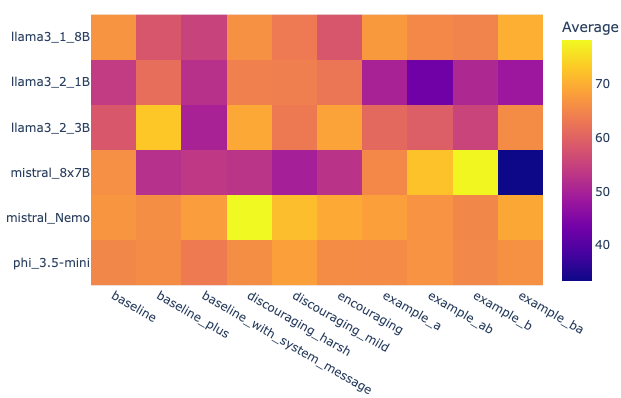
\includegraphics[width=\columnwidth]{img/model_performence_on_prompts.png}
  \caption{Models performance on all prompts}
  \label{rep: Models average heatmap}
\end{figure}

\subsection{Analyzing Model Confidence through Logit Differences}

\begin{figure*}[htbp!]
  \centering
  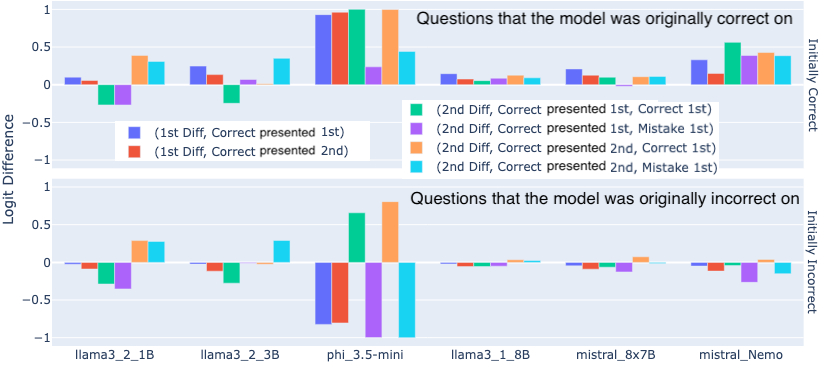
\includegraphics[width=\textwidth]{img/model_confidence_by_initial_correctness_on_baseline.png}
  \caption{Model's confidence in each of the 6 confidence samples, on the baseline prompt. The top row represents the models' were correct in their initial response, while the bottom row represents the models' were incorrect in their initial response.}
  \label{fig:models_confidence_per_initial_correctness}
\end{figure*}

\paragraph{}

In the previous experiments, we focused on accuracy based metrics to evaluate the models' performance. However, the way that models produces their answers is not binary, and using only accuracy as a metric may not provide a full picture of the models' decision-making process. In this experiment, we aim to analyze the models' confidence in their answers by examining the difference in logits between the correct and incorrect answer tokens. By analyzing the confidence shifts after expressing doubt, we assess the models' ability to adjust their internal certainty and correct their answers.

For each question, we sampled the confidence (logit difference between the correct and incorrect answer tokens) at 2 points, as marked in the baseline template \ref{fig:baseline_prompt_template}, \textbf{Point A} (1st response / before doubt) and \textbf{Point B} (2nd response / after doubt).

In \textbf{Point A}, models can either answer \textbf{a} or \textbf{b} as their initial response. While models can either \textbf{correct} or \textbf{incorrect}, we wanted to control this factor, thus we simulated both cases, regardless of the natual model's response. so in fact, for each question, we sampled 3 logit differences, one in \text{Point A} and two in \text{Point B}, one for each case of the model's initial response.
In addional, based on the results of the previous experiment, we found out that the answer positioning has a significant impact on the models' performance. Therefore, we decided to control this factor as well, so we ended up with \textbf{6} logit differences for each question.

\paragraph{Experimental Setup}

\begin{itemize}
  \item Number of questions: 1,500
  \item \textbf{Experiment Scenarios}:
    \begin{itemize}
      \item \textbf{Correct Answer Position}: Correct answer positioned at \textbf{a} or \textbf{b}.
      \item \textbf{First Response}: Initial response is correct or mistaken.
    \end{itemize}
  \item \textbf{Evaluation Metrics}:
    \begin{itemize}
      \item \textbf{Baseline Confidence}: Confidence at Point A (initial response).
      \item \textbf{Adjusted Confidence}: Confidence at Point B (after expressing doubt).
      \item \textbf{Change in Confidence} ($\Delta$ Confidence): Difference between adjusted and baseline confidence.
    \end{itemize}
\end{itemize}

\paragraph{Results and Discussion}

Figure~\ref{fig:models_confidence_per_initial_correctness} illustrates the average confidence for each model across the 6 confidence samples, separated by the initial response correctness. Figure~\ref{fig:models_confidence} illustrate the distribution of the confidence in the second response, in relation to the initial response.
\begin{itemize}
  \item \textbf{Size do matter}: We can see that that llama3.2 3B is almost always the better than the 1B model. And that high a postive sign for the correctness of the response.
  \item \textbf{Confidence Shifts}: We observed that models generally exhibited a change in confidence after expressing doubt.
\end{itemize}

\begin{figure*}[ht!]
  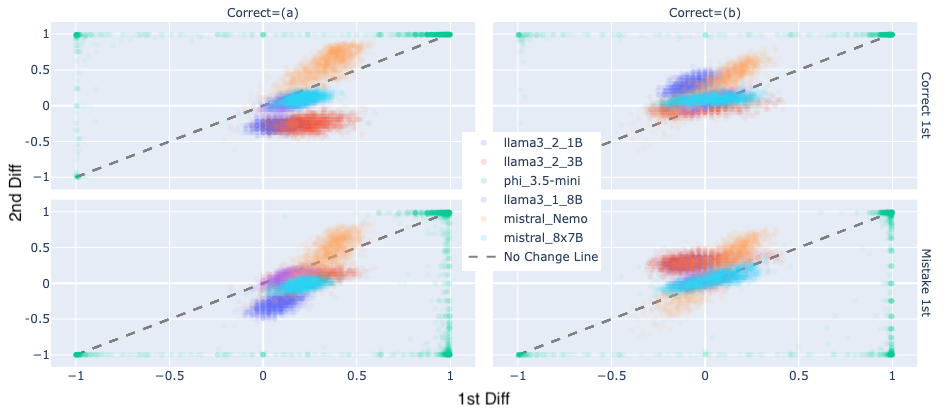
\includegraphics[width=\textwidth]{img/first_vs_last_logit_diff_on_baseline_copy.png}
  % 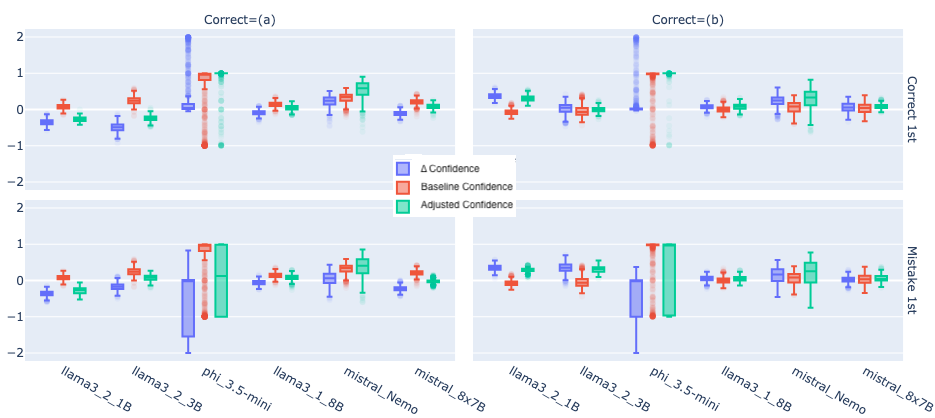
\includegraphics[width=\textwidth]{img/confidence_distribution_on_baseline.png}
  \caption{Model Confidence distribution on the baseline prompt, columns represent whether the correct answer was positioned first or second, and rows represent the models' initial response correctness.}
  \label{fig:models_confidence}
\end{figure*}

\subsection{Repeated Doubt with Feedback}

Building on the results of previous experiments, which showed no consistent or significant improvement in model accuracy when doubt was introduced, this experiment investigates whether adding feedback on the model's performance after expressing doubt, combined with iterative repetition, can enhance accuracy.

\paragraph{Experimental Setup}
The experimental setup was consistent with the first experiment, using the same set of models and evaluation methodology. The procedure was as follows:

\begin{enumerate}
  \item The model was presented with factual questions, each with two possible answers. After selecting an answer, doubt was expressed regarding the model's choice.
  \item After the model refined its answer in response to the expressed doubt, feedback was provided indicating whether its answer was correct both before and after the doubt stage.
  \item This process was repeated over five iterations to observe whether performance improved over time.
\end{enumerate}

To manage computational constraints, each model underwent 1,000 repetitions of this iterative process. To assess whether feedback influenced accuracy, we compared these results to a similar iterative process without performance feedback.

\paragraph{Results and Discussion}
The results of this experiment are presented in figure \ref{rep: graph}. In addition, an ANOVA test was conducted to asses the statistical significance of the effects of doubt, feedback, and iteration on accuracy. Table \ref{rep: p-value} summarizes the p-values for each factor across the tested models. Significant effects (p-value < 0.05) are highlighted in bold.

\begin{figure*}[h!]
  \centering
  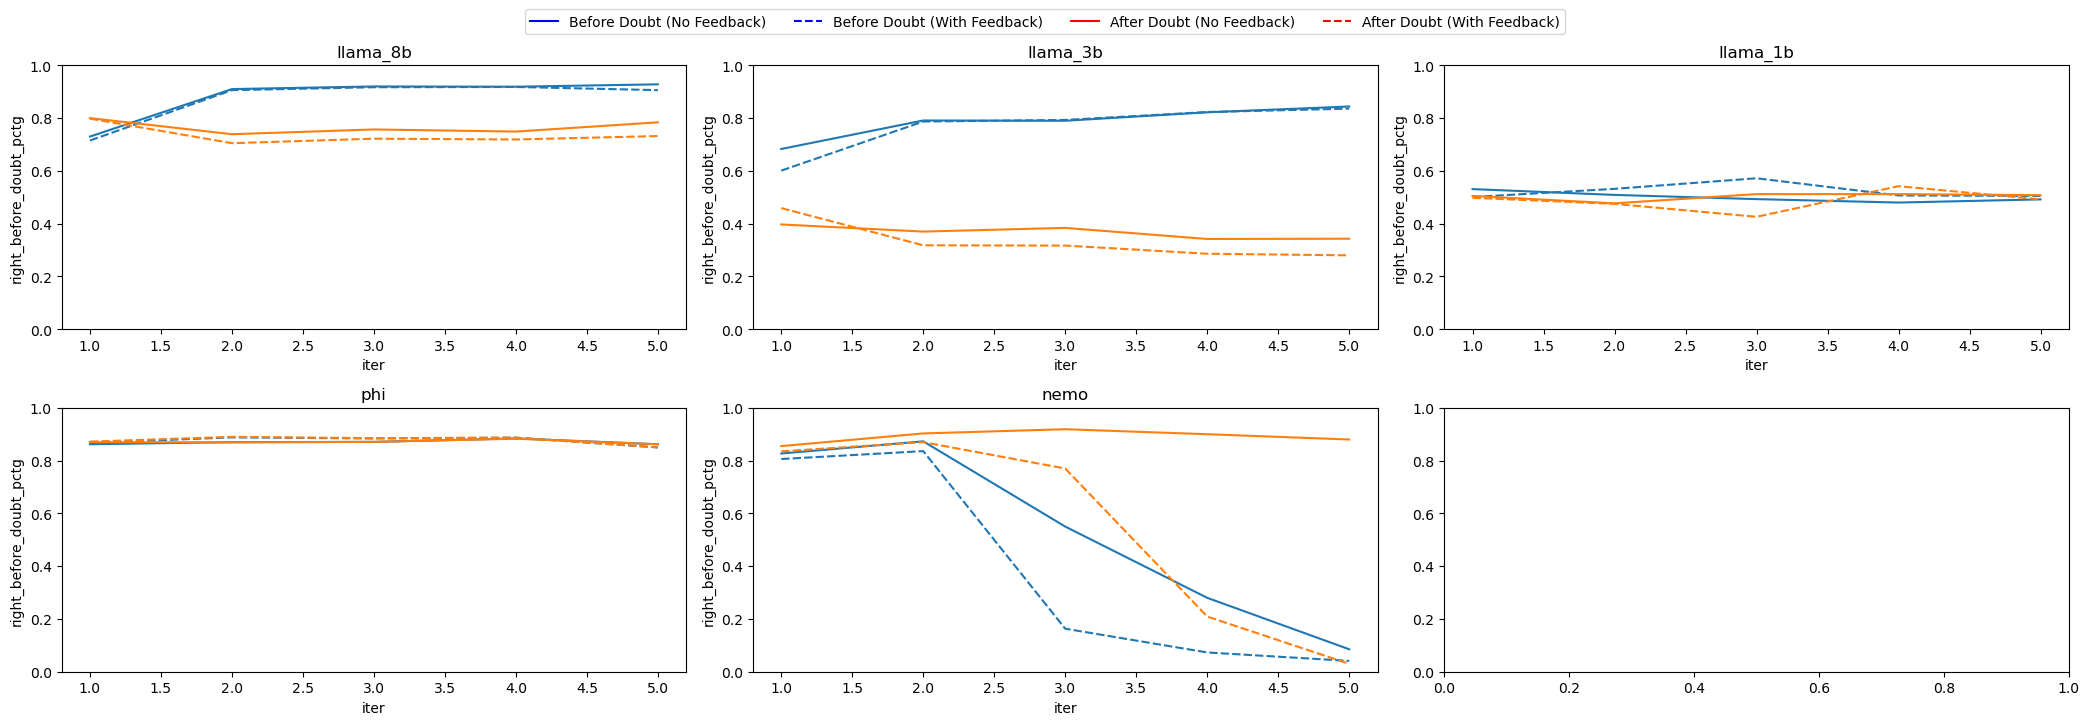
\includegraphics[width=\textwidth]{img/repeted_graph.png} % Replace with your image file name
  \caption{Model accuracy across iterations, separated by conditions: before/after doubt and with/without feedback.}
  \label{rep: graph}
\end{figure*}

\begin{table}[ht]
  \centering
  \small
  \begin{tabular}{|l|l|l|l|l|}
    \hline
    \textbf{Model} & \textbf{Size} & \textbf{Doubt} & \textbf{Feedback} & \textbf{Iteration} \\
    \hline
    Llama 3.2 & 1B & 0.21 & 0.81 & 0.95 \\
    Llama 3.2 & 3B & \textbf{0.0001} & 0.1 & 0.46 \\
    Phi 3.5 & 3.82B & 0.72 & 0.17 & \textbf{0.01}\\
    Llama 3.1 & 8B & \textbf{0.0001} & \textbf{0.002} & \textbf{0.0001} \\
    Mixtral & 8x7B & & & \\
    Nemo & 12.2B & \textbf{0.02} & \textbf{0.03} & \textbf{0.01}\\
    \hline
  \end{tabular}
  \caption{P-values from ANOVA tests for the effects of doubt, feedback, and iteration on accuracy for each model. Bold values indicate significance (p-value < 0.05).}
  \label{rep: p-value}
\end{table}

These results reveal varied responses to doubt, feedback, and iteration across different LLM architectures:

\begin{enumerate}
  \item \textbf{Larger Llama Models (3B and 8B):}
    \begin{itemize}
      \item Doubt negatively impacted accuracy. A possible reason for that may be that the doubt reduces model's confidence in its answers, thus confusing it.
      \item Iterative questioning led to performance improvements at the pre-doubt stage (i.e before the doubt was induced), suggesting that a preliminary "warm-up" phase could be beneficial.
      \item To test the necessity of doubt during warm-up, we conducted an additional experiment with Llama-8B, iteratively questioning it without inducing doubt. We chose to focus on Llama-8b because table \ref{rep: p-value} shows that the effect of iterative questioning on accuracy is statisticaly significant for this model. The results (Figure \ref{rep: graph_8b}) indicate that iterative questioning alone achieves similar improvements, showing that induced doubt is unnecessary in the suggested warm-up step.
    \end{itemize}
  \item \textbf{Stable Performance (Phi, Llama 1B):}
    \begin{itemize}
      \item These models exhibited stable performance, unaffected by doubt, feedback, or iterative processes.
    \end{itemize}
  \item \textbf{Nemo Model:}
    \begin{itemize}
      \item Doubt had no significant impact during the first iteration, but subsequent iterations revealed an intriguing pattern: accuracy decreased in the pre-doubt stage but improved post-doubt.
      \item A possible explanation may be that the model anticipate the doubt prompt and intentionally adjust its answers. However, when feedback was added, performance degraded also after the doubt is induced.
    \end{itemize}
\end{enumerate}
% \begin{itemize}
%     \item In the larger Llama models (3B and 8B) doubt reduces model accuracy. A possible reason for that may be that the doubt reduces model's confidence in its answers, thus confusing it. However, iteratively asking the models questions may lead to an improvement whenever doubt is not induced. This may advise for performing a "warm-up" round before asking the model a question. To check whether the induced doubt is necessary at this warm-up stage, we have conducted further experiment on Llama-8b, asking it questions in iterative manner, without adding doubt. We chose to focus on Llama-8b because it is shown with statistical significance that iterative questioning improves its performance. The results of this experiment are presented in Figure \ref{rep: graph_8b} and teach us that even  without the induced doubt, same improvement over iterations is achieved, thus leading to the conclusion that the induced doubt does not effect the improvement seen via iterative questioning, ans is therefore not necessary for the warm-up step suggested above.

%     \item In some of the models (phi, Llama 1B) it seems that the performance is stable and not influenced by doubt, feedback, or iterative process.

%     \item In Nemo model, it seems that the doubt does not improve model performance at the first iteration. However, the iterative process causes an interesting phenomenon where the model performance degrades at the pre-doubt stage, while staying good, and even improves a bit, after doubt is induced. A possible explanation may be that the model intentionally making mistakes in the pre-doubt stage, aligning with the expected doubt that it predicts should come, and then improves its answer after the doubt is induced. Interestingly, when provided with feedback, the model losses performance also after the doubt is induced.

% \end{itemize}

\begin{figure}[ht!]
  \centering
  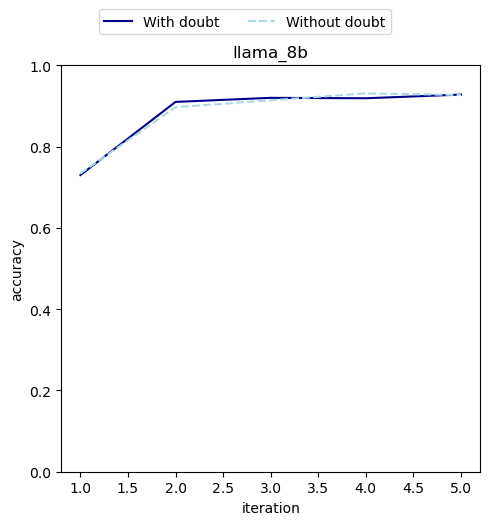
\includegraphics[width=\columnwidth]{img/llama_8b_graph.png} % Replace with your image file name
  \caption{Llama-8B accuracy across iterations with and without induced doubt. For the experiment with doubt, accuracy before the doubt stage is reported, consistent with the blue line in Figure \ref{rep: graph}.}
  \label{rep: graph_8b}
\end{figure}
